\section{Summary}
This chapter will present the change detection problem for targets concealed by a forest. It will 
also present the SAR system that was used to perform the data acquisition and the dataset that was created by this system.
The dataset consists of SAR images collected that the Swedish low VHF-band SAR system CARABAS-II. 
The images were made publicly available by the Swedish Airforce Research center with the purpose of fostering research on the 
subject field of target detection under tree foliage. 


\section{Wavelength Resolution SAR Systems}
Wavelength resolution SAR images are radar systems with resolution in the order of 
the radar system Wavelength. According to \cite{62}, the resolution of a cell of a SAR image can be
calculated by:

\begin{equation}
    \delta = \frac{\lambda_c c}{4 \theta_H B}
\end{equation}

where $\lambda_c$ is the wavelength corresponding to the radar central frequency, $\theta_H$
is the aperture angle (in radians), $c$ is the speed of light and $B$ is the system bandwidth.

It is obvious that the backscatter characteristcs of the SAR depends on the frequency band of the system.
For wavelength-resolution SAR systems there is a significant difference between the backscatter of targets with size the order
of the wavelength - which present the resonance scattering phenomena \cite{63} - and targets small compared to the wavelength - which present
the the Rayleigh scattering phenomena \cite{63}. 

According to (17ref), Wavelength SAR systems are not sensitive to small scatterers inside the resolution cell,
thus the scattering process is mainly due to scatterers with dimensions in the order of the system wavelength.
Since the resolution of the cell is similar to the resolution of the scatterer, there can be only one single scatterer inside each cell, 
therefore the image will not be greatly affected by speckle noise (speckle noise is a major cause of problems in non wavelength-resolution SAR still). For example, according to \cite{64}
in frequencies below 100 MHz, in forest areas, the backscatter is dominated by backscattering from tree foliage.

Moreover, scatterers that are large tend to be static objects, hence a stack of images of the same area will present a high degree of 
similarity between multi-pass acquisitions. Therefore regular noise redution techniques do not have to be applied when dealing with those set of images \cite{ 61}.

It is also worth mentioning that according to \cite{ 66}, signal attenuation in low-frequency wavelength-resolution SAR systems 
is not a major concern. Studies \cite{63} have also shown that signal attenuation can be as little as 3dB in low-frequency SAR acquisitions in forest areas.


Due to all that, according to (63ref), low resolution SAR systems are better suited to Foliage Penetrating (FOPEN) applications.
Also according to (63ref), VHF-band is the optimal radar system for FOPEN applications for vehicle-sized target detection.

\section{The CARABAS-II Challenge Problem}
There are many situations were there is a need for monitoring vehicles concealed by foliage over a large area.
For example, for military applications, it might be necessary to monitor the positioning of enemy vehicles trespassing
a restricted area. For environmental purposes it might be needed to pinpoint the position of vehicles that are being used
for illegal deforestation over protected forests. If SARs are to be used for such purposes, it is ideal that low frequency systems
are chosen since those provide a wide survaillance area and good foliage penetration capabilities. 
At low frequency (VHF-band) the main backscatter from the target area is due to large scatterers, e.g. tree canopy, houses,
vehicles, and other man-made objects, which will appear as very bright objects in the image.

The challenge related to change detection is associated with the trade-off between having high accuracy detection and high false alarm rate.
Normally what happens is by trying to increase the overall accuracy of detection algorithms will incur in having a high number of false alarms, 
therefore when designing an algorithm for detection it is necessary to have both good detection capabilities and a low enough false alarm rate
to be used by the client. In foliage penetration applications, the main source of clutter comes from large tree trunks, and the more sparse the
forest is the less will be the number of false targets. It is also true that the larger the tree then the higher will be the number of false alarms \cite{Book_ML}.

The objects that will be used to assess the quality of the change detection method will be a set of 25 military vehicles distributed among a testing area.
Since those objects are large (compared to the bandwidth of the signal), and stationary, then their radar signature will be very stable between acquisitions.
This will be used as an advantage by taking acquisitions with different flight passes to supress clutter noise from tree canopy.

According to (ref 1/2 challenge) VHF-band has good performance for detecting targets under trees, but there are very few VHF SAR systems in the world.
To overcome this problem researchers from the FOI released a VHF-band SAR image dataset to the public to foster the developement of 
change detection methods for wavelengh-resolution SAR systems in VHF band, which is the dataset that will be used in this work.


\section{The CARABAS-II System}

The CARABAS-II is the second generation SAR system designed by the Swedish Defense Research Agency (FOI) for FOPEN applications.
The CARABAS-II has participated in numerous military campaigns and has been used for reasearch purpose since the nineties.
The radar is a VLF UHB SAR system that transmits HH-polarized radio waves in the frequency range of 
20-90 MHz, therefore having resolution in the range of 3.3-15 m. The radar antenna is mounted on a Sabreliner aircraft as seen in \figref{fig:sabreliner}.

\begin{figure}[h]
    \centering
    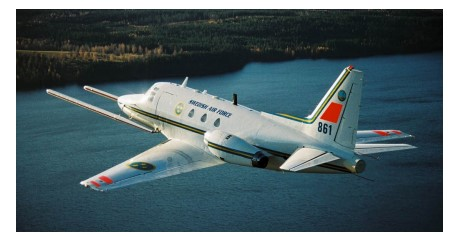
\includegraphics{chapter6/sabreliner.jpg}
    \caption{The CARABAS-II VHF SAR mounted in front of a Sabreliner airplane}
    \label{fig:sabreliner}
\end{figure}

In the table below the system parameters for the CARABAS-II system are presented for the
flight campaigns that were used in this work. 

\begin{table}[h]
    \centering
    \begin{tabular}{|c|c|}
        \hline
        System Parameters & Values \\ \hline
        Nominal flight altitude & 3 - 9 km \\ \hline
        Nominal flight speed & 127 m/s \\ \hline
        Frequency band & 20-86 MHz \\ \hline
        Aperture angle & 90 degrees \\ \hline
        Transmitted power & 500 W \\ \hline
        Pulse modulation & Non-linear frequency modulation \\ \hline
        Radio Frequency Interference (RFI) sniff & On \\ \hline
        Frequency sub-bands & 35 (36 with RFI-sniff \\ \hline
        Frequency step & 1.875 Mhz \\ \hline
        Center frequencies & 21.25-85Mhz \\ \hline
        Pulse repetition & frequency 5000Hz \\ \hline
        Pulse length & 15$\mu$s \\ \hline
        Maximum range & 26.4 km \\ \hline
    \end{tabular}
    \caption{CARABAS-II SAR system parameters. Source: (76 ref)}
    \label{tab:carabas_system}
\end{table}

\section{The CARABAS-II Dataset}

By trying to promote research on change detection algorithms for wavelength-resolution
images, FOI created a dataset of images acquired by CARABAS-II and made it publicly available. 
This dataset is the one used to test and assess the quality of the proposed CDA.

The dataset consists of 24 SAR images selected from over 150 images obtained during different flight campaigns.
Each image covers the same ground area of 6 $km^2$ (3 km vertically and 2 km horizontally)
and is given in the form of a 3000 X 2000 matrix, where each pixel size is 1km x 1km.
According to \cite{ 77,62,78} the images are already calibrated, pre-processed and geocoded.

The location of the image dataset is inside the military base station Missile Test Area North
Vidsel in northern Sweden in 2002. The test site is a region near the village of Nausta \cite{ 75}.
The vegetation of the area is dominated by Scots Pine tree \cite{ 76}, which consists of small and medium size trees.
According to \cite{75} the area also contains fields, roads and lakes.

With the objective of testing CDA quality, it was deployed 25 testing targets over the testing with different configuration 
and arrangements. The testing targets consists of ten TGB11 model military vehicles, eight TGB30 model 
military vehicles, and seven TGGB40 model military vehicles. The dimensions of each vehicle are presented in the table (numero).
From the table (numero) it can be seen that the dimensions of the vehicles are similar to the wavelength of the CARABAS-II system,
therefore all advantages of targets with similar dimension to the wavelength previously mentioned hold true for the dataset.

\begin{table}[h]
    \centering
    \begin{tabular}{|c|c|c|c|c|}
        \hline
        Military Vehicle & Lenght & Width & Height & Quantity \\ \hline
        TGB11 & 4.4 m & 1.9 m & 2.2 m & 10 \\ \hline
        TGB30 & 6.8m & 2.5m & 3.0 m & 8 \\ \hline
        TGB40 & 7.8m & 2.5m & 3.0m & 7 \\ \hline
    \end{tabular}
    \caption{Target dimensions}
    \label{tab:vehicle_dimensions}
\end{table}


The dataset of 24 images were acquired using four different flight passes. Each 
flight pass has an incidence angle of 58 degrees, used the StripSAR mode and was acquired with the radar looking left \cite{ 75,76}.
The vehicles were positioned in two diferent forests, Forest 2 being in the northwest of the field, and forest 1 being in the
southeast of the test area. 

\begin{figure}[h]
    \centering
    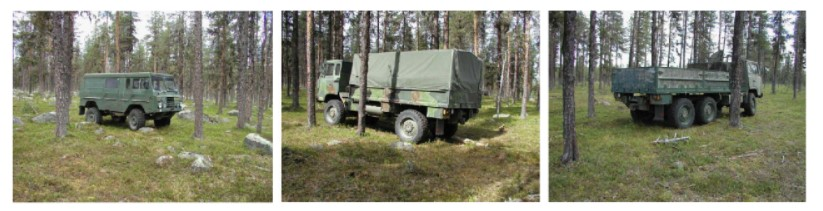
\includegraphics{chapter6/carabas_vehicles_fisico.jpg}
    \caption{Military vehicles used as target. Left:TGB11. Middle:TGB30. Right:TGB40. 
    This picture also depicts the vegetation characteristics of the test area}
    \label{fig:veiculos}
\end{figure}

The vehicles in mission 2 are positioned in forest 2 and have a heading angle of 225 degrees pointing southwest direction;
vehicles in mission 3 are positioned in forest 2 and have a heading angle of 315 degrees pointing northwest direction;
vehicles in mission 4 are located in forest 1 and have the same heading angle of mission 2;
vehicles in mission 5 are located in forest 1 and have a heading angle of 270 degrees pointing west direction.
Vehicles in mission 2 and 3 are separated approximately by 50m, as such for vehicles in mission 4 and 5.
\figref{fig:carabas_vehicles} presents images of each mission with the vehicles area highlighted in red.

\begin{figure}[h]
    \centering
    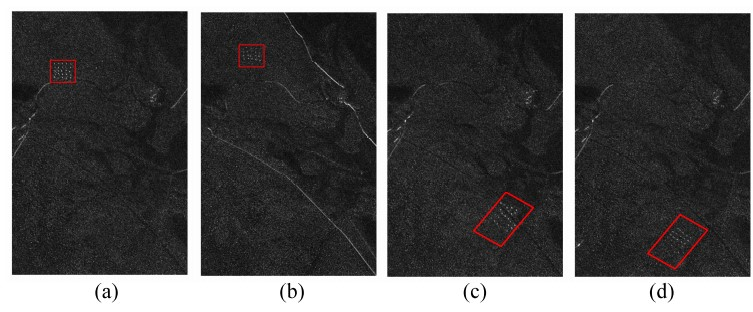
\includegraphics{chapter6/carabas_vehicles.jpg}
    \caption{Examples of CARABAS-II images where (a) is mission 2, (b) is mission 3, (c) is mission 4 and (d)
    is mission 5}
    \label{fig:carabas_vehicles}
\end{figure}

In table \ref{tab:flight_mission} it is presented the summary with the information of each image in the dataset

\begin{table}[H]
    \centering
    \begin{tabular}{|c|c|c|c|c|}
        \hline
        Image Number & Mission & Pass & Flight Heading (degrees) & Target Heading \\ \hline
        1 & 2 & 1 & 225 & 225  \\ \hline
        2 & 2 & 2 & 135 & 225  \\ \hline
        3 & 2 & 3 & 225 & 225  \\ \hline
        4 & 2 & 4 & 135 & 225 \\ \hline
        5 & 2 & 5 & 230 & 225 \\ \hline
        6 & 2 & 6 & 230 & 225 \\ \hline
        7 & 3 & 1 & 225 & 315 \\ \hline
        8 & 3 & 2 & 135 & 315 \\ \hline
        9 & 3 & 3 & 225 & 315 \\ \hline
        10 & 3 & 4 & 135 & 315 \\ \hline
        11 & 3 & 4 & 135 & 315 \\ \hline
        12& 3 & 6 & 230 & 315  \\ \hline
        13 & 4 & 1 & 225 & 225  \\ \hline
        14 & 4 & 2 & 135 & 225  \\ \hline
        15 & 4 & 3 & 225 & 225  \\ \hline
        16 & 4 & 4 & 135 & 225  \\ \hline
        17 & 4 & 5 & 230 & 225  \\ \hline
        18 & 4 & 6 & 230& 225 \\ \hline
        19 & 5 & 1 & 225 & 270  \\ \hline
        20 & 5 & 2 & 135 & 270  \\ \hline
        21 & 5 & 3 & 225 & 270  \\ \hline
        22 & 5 & 4 & 135 & 270  \\ \hline
        23 & 5 & 5 & 230 & 270  \\ \hline
        24 & 5 & 6 & 230 & 270  \\ \hline
    \end{tabular}
    \caption{Measurements parameters for each image}
    \label{tab:flight_mission}
\end{table}

\section{Traditional Change Detecion in Wavelength-Resolution SAR Images}

The field of FOPEN target detection using wavelength-resolution SAR images (both in VHF and UHF bands) has been 
around of decades \cite{ 25,48,79,80}. Among those studies, the CARABAS-II system dataset was used in many different FOPEN studies 
\cite{}. 

As previously mentioned, the objective of the study is to create a change detection method that will compare 
different images of the same target field (in this case, the forests in Sweden) and try to identify the targets that 
have changed position in the image (in this case, the military vehicles TGB11, TGB30 and TGB40 ) and give the exact location of the vehicle positions.


There are several change detection methods that were already used in the CARABAS-II dataset.
The first method that yielded accuracy high enough for real world applications was based in Bayes linear classification \cite{81}.
After that, a myriad of new methods were proposed, such as: Likelihood-ratio test (LRT) \cite{ 61}, combination of LRT and Space-Time 
adaptative processing (STAP) \cite{ 76} among others. Traditionally CDAs were also mainly based on traditional statistical decision theory, e.g., 
traditional hypothesis testing criterion methods, such as maximum a posteriori 
criterion \cite{Book_Kay}, likelihood ratio test \cite{LRT1,LRT2,LRT3}, generalized likelihood ratio test \cite{GLRT1,GLRT2,GLRT3}, 
or Bayesian theory approaches \cite{Bayes1, Bayes2}. Several of those CDAs have achieved high accuracy 
in terms of true positives, but most show unsatisfactory performance in terms of false positives percentage \cite{Carabas, Ricardo,LucasRamos,Chris}.





